El algoritmo que se utilizó para obtener las soluciones es \texttt{Produce-and-Choose}, cuenta con 
dos fases.
En la primer fase se generan cierta cantidad de bundles, e la fase siguiente se seleccionan los 
bundles que serán parte de la solución.\\
A continuación se explican los algoritmos utilizados para cada fase.
\section{Generación de bundles}
Dado un conjunto de papers el objetivo es generar clusters en los cuales los papers suficientemente similares pertenescan al mismo cluster
y en cluster distintos los dicimiles. Cuanto mayor es la similitud en el cluester (intra) y mayor la diferencia entre los cluster (inter) 
es mejor la clusterización.
Definir como se consituye un cluster es complejo. Por ejemplo para los 20 puntos que se muestran a continuación existen tres (o más) formas de clusterizar
que son validas. Entonces la mejor definición depende del tipo de dato y del resultado esperado.

\begin{figure}[H]
  \centering
    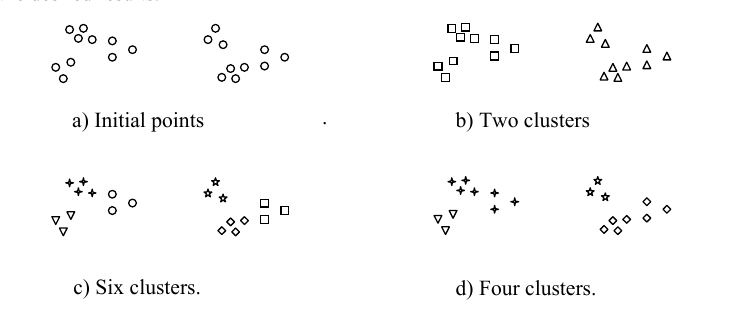
\includegraphics[width=0.3\textwidth]{img/howToCluster.png}
  \caption{Agregar descripcion}
  \label{res:img-howToCluster}
\end{figure}

En la clusterización para Composite Retrival, la definición es generar cluster máximizando el costo que esta acotado por el budget.
Ya que lo esperado es obtener cluster que utilicen el máximo del presupuesto.\\

El problema de la clusterización es NP-hard (agregar ref, explicar problema de clusterizacion),
por lo que se utilizaron dos técnicas ya conocidas para aproximarse a una solución.\\
La principal diferencia entre las estrategias de clusterización es entre la jerarquica y de partición.
La primer técnica produce un árbol de particiones, la raíz es un cluster que contiene todos los items
y las hojas son clusters con un único item. Cada nivel intermedio, puede ser visto, como la combinación
entre entre dos clusters del nivel inferior inmediato. Mientras que la segunda genera solo un nivel de las particiones de los items de una vez.\\ 
Se implmentaron las dos técnicas para la clusterización la jerarquica con el algoritmo
Hierarchical clustering y la de partición con Bundles One-By-One.\\

\subsection{Bundles One-By-One}
La herurística \texttt{BOBO-x} en cada paso se elige un item, denominado pivote, se genera un bundle a partir del pivote. 
El parámetro $x$ define la cantidad de bundles a generar. El caso de que $x$ sea 'Ex' todos los itmes son pivotes.\\
\subsection{Hierarchical clustering}
La heurística Hierarchical clustering \texttt{HAC} 
se define la función de distancia entre clusters comienza con tantos clusters como cantidad de elementos, cada uno está 
conformado por un solo ítem y en cada paso se unen los dos clusters más cercanos que respetan las restricciones. 
Para ello se define la función de distancia para los items $u$ y $v$ como:\\
\begin{equation}
d_{1}(u,v) = 1 - s(u, v)
\end{equation}

Con la función de distancia $d_{1}$ en la clusterización se generan los cluster lo más cohesivos posibles,
En la figura 1 se observa que el algoritmo selecciona los items más cercanos. En las búsquedas que se realizan en composite ...
se tiene el parámetro $\gamma$ que indica que tipo de resultado es el esperado. 

\begin{figure}[H]
  \centering
    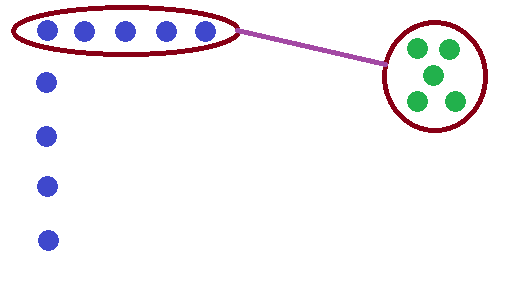
\includegraphics[width=0.3\textwidth]{img/cluster2.png}
  \caption{Selección de bundles usando $d_{1}$}
  \label{res:img-usingEfficientHAC}
\end{figure}

En caso de que el $\gamma$ sea pequeño, la 
clusterizacion esperada para la misma instncia es la que se visualiza en la imágen 2, clusters no tan cohesivos pero más variados.
Por lo que se define una función de distancia que considera el $\gamma$.\\
\begin{equation}
d2(u,v) = 1 - FO(\{u\} \cup \{v\})
\end{equation}
Donde $FO$ es la función definida en \eqref{eq:fnObj} \\

\begin{figure}[H]
  \centering
    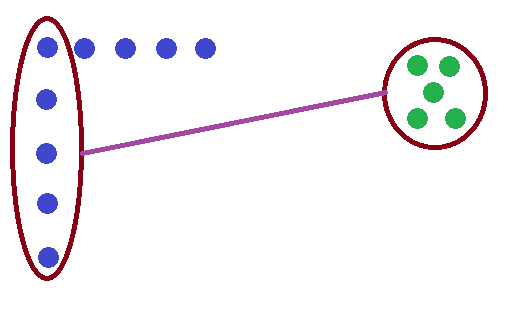
\includegraphics[width=0.3\textwidth]{img/cluster1.png}
  \caption{Selección de bundles usando $d_{2}$}
  \label{res:img-usingSingleHAC}
\end{figure}

Para la distancia $d_{1}$ se implementó el algoritmo \texttt{EfficientHAC} que es tiene una 
complejidad $\mathcal{O}(n^{2})$, mientras que para $d_{2}$ el algoritmo es \texttt{SingleHAC} que 
la complejidad es $\mathcal{O}(n^{2} * \ln{n})$. Según se demostró en el capítulo 17 de 
\cite{informationRetrival}


\section{Selección de bundles}
Al finalizar la producción de bundles, se deben seleecionar los $k$ bundles para la solución.
El problema de seleccionar los bundles que maximizan la función objetivo, se traduce en 
encontrar en el grafo G el k-subgrafo de mayor peso de nodos y aristas.

Se implementó el algoritmo que propone ``Composite ...''\cite{compositeRetrival} que transforma el 
grafo G 
en el grafo G', con los mismos nodos y aristas, redefiniendo el peso de las aristas con la función:\\

\begin{equation}
\omega_{1}(u,v) = \dfrac{\gamma}{2( k - 1)} (\omega(u) + \omega(v)) + (1 - \gamma)\psi(u,v) 
\end{equation}

(aca va el algoritmo)\\

En la función $\omega_{1}(u,v)$ el valor de la función $\psi(u,v)$  es considerablemente menor al de
$\omega(u) + \omega(v)$, (en el intra se suma los ejes de todos los nodos, el inter es el máximo entre los items)
implica que $\gamma$ no cumple con el objetivo de balancear entre una solución cohesiva y una variada.
Para esto se funciones $\omega$ alternativas.\\

Con $\omega_{2}(u,v,w,y)$ la búsqueda se realiza con la combinación de cuatro nodos, por lo que el orden de complejidad
aumenta a ...

\begin{equation}
\begin{split}
\omega_{2}(u,v,w,y) &= \dfrac{\gamma}{2( k - 1)} (\omega(u) + \omega(v) + \omega(w) + \omega(y)) \\
&+ (1 - \gamma)(\psi(u,v) + \psi(u,w) + \psi(u,y)  + \psi(v,w) + \psi(v,y) + \psi(w,y))
\end{split}
\end{equation}

La función $\omega_{3}(u, k)$ recibe $u$ el conjunto de clusters seleccionados hasta el momento 
y $k$ que es la cantidad de cluesters para la solución. Con $k$ y el tamaño de $u$ se calcula el 
coeficiente con el propósito en que en cada paso se pondere el inter y el intra. Para eso se multiplica
con coeficientes cada parte de la función. Con esto se mantiene la relación de inter e intra durante la selección de bundles

\begin{equation}
\begin{split}
\omega_{3}(u,k) &= \dfrac{k}{u.size} * (\gamma \sum_{v \in U}(w(v))) \\
&+ \dfrac{(k * (k-1))}{2} * \dfrac{2}{(u.size() * (u.size() - 1))} * 1 - \gamma \sum_{v,w \in U}(\psi(v,w))
\end{split}
\end{equation}

\begin{algorithm}[H]
\begin{algorithmic}[1]
\REQUIRE $produced:Vector<SnowFlake>, numRequested:Integer$
\ENSURE $selected:Vector<SnowFlake>$.
\STATE $selected:Vector<SnowFlake> \leftarrow []$
\STATE $originalSize:Integer \leftarrow produced.size$
\WHILE {$selected.size < numRequested\ AND\ selected.size < originalSize$}
\STATE $selectedTemp \leftarrow selected$
\STATE $(candidateOne, candidateTwo) \leftarrow (i, j)\ where$ \\ 
$\displaystyle\max_{i \neq j} (FO(selectedTemp.push(produced_{i} \cup produced_{j})))$
\STATE $produced.erase(i)$
\STATE $produced.erase(j)$
\STATE $selected.push(candidateOne)$
\STATE $selected.push(candidateTwo)$
\ENDWHILE
\RETURN $selected$
\end{algorithmic}
\caption{Selección de bundles de a pares}\label{alg:algSelTuple}
\end{algorithm}
\subsection{Selección proporcional}
Además como tercera opción de selección se implementó un algoritmo proporcional que en cada paso se 
ponderan los resultados de la función que calcula el intra y el inter restante, intentando 
\textquotedblleft adivinar\textquotedblright  el valor de las próximas iteraciones y de esta manera 
dar más importancia en los primeras iteraciones al valor del inter.
\begin{algorithm}[H]
\begin{algorithmic}[1]
\REQUIRE $produced:Vector<SnowFlake>, numRequested:Integer$
\ENSURE $selected:Vector<SnowFlake>$
\STATE $w(u) = \dfrac{k}{u.size} * (\gamma \sum_{v \in U}(w(v))) + \dfrac{(k * (k-1))}{2} * \dfrac{2}{(u.size() * (u.size() - 1))} * 1 - \gamma \sum_{v,w \in U}(\psi(v,w))$
\STATE $available \leftarrow produced$
\STATE $selected \leftarrow []$
\WHILE {$selected.size < numRequested\ AND\ selected.size < produced.size$}
\STATE $candidate \leftarrow max_{i}$
\ENDWHILE
\RETURN $selected$
\end{algorithmic}
\caption{Selección de bundles proporcional}\label{alg:algSelProp}
\end{algorithm}

\section{Modificación de PAC para búsquedas específicas}
Para la obtención de la solución se modificó la producción de bundles como así también la 
selección de los mismos (Produce and Choose). \\
En la producción de bundles en el algoritmo jerárquico, se utilizó la similitud del perfil 
específico con los papers en cada paso que intenta unificar dos clusters. A diferencia del cálculo 
original que la compatibilidad de dos nodos esta dada por su distancia previamente obtenida, en 
este nuevo caso se agrega a ese resultado la compatibilidad de cada uno de ellos con el perfil 
específico. \\
Para la producción del algoritmo BOBO, se agregó junto al pivote en todos los clusters. \\
Para la selección de los bundles que formarán parte de la solución, a cada cluster se le 
calculo el valor intra también se tuvo en cuenta la similitud de todos los elementos con el perfil  
específico, de esta manera a los clusters que contenían papers con los mismos tópicos que el del 
vector especifico se le dio mayor peso.

\section{Heurística golosa para la obtención de una solución}
En todas los algoritmos previos se centraron en, primero construir buenos bundles maximizando solo 
el valor propio de cada bundle, o sea, el valor inter bundle. Una vez generado los suficientes 
\textquotedblleft buenos\textquotedblright  para luego seleccionar dependiendo de la 
estrategia elegida la solución final, ahora si, maximizando la función objetivo propuesta 
originalmente.\\
Para este heurística golosa propusimos ir construyendo los bundles finales teniendo en cuenta en 
cada paso la función objetivo, esto es, en cada paso cuando se intenta agregar un nuevo elemento a 
un bundle se calcula su valor total de la función y se evalúa en que bundle conviene agregarlo. 
Esto se repite para todos los items, haciendo que cuando tengo que agregar un nuevo ítem a la 
solución ya calculé para todos los items que no se encuentran en la solución en que bundle conviene 
agregarlo y cual es el valor de la función en ese caso, quedándonos siempre con el mejor valor 
posible.
\begin{algorithm}[H]
\begin{algorithmic}[1]
\REQUIRE $numOfSnowFlakes:Integer$
\ENSURE $selected:Vector<SnowFlake>$
\STATE $selected_{i}:Vector<SnowFlake> \leftarrow \emptyset_{0\leq i<numOfSnowFlakes}$
\STATE $isComplete:Bool \leftarrow False$
\STATE $elements:Set<Element> \leftarrow ElementsOfTheProblem$
\WHILE {$isComplete == False$}
\STATE $bestScore:Double \leftarrow -\infty$
\STATE $bestElement:Element \leftarrow \varnothing$
\STATE $bestBundle:SnowFlake \leftarrow \varnothing$
\FOR {$elem:Element \in elements$}
\FOR {$bundle:SnowFlake \in selected$}
\IF {$isValidBundle(bundle \cup \{elem\}) == True$}
\STATE $score:Double \leftarrow FO(selected.replace(bundle, bundle \cup \{elem\}))$
\IF {$score > bestScore$}
\STATE $bestScore \leftarrow score$
\STATE $bestBundle \leftarrow bundle$
\STATE $bestElement \leftarrow elem$
\ENDIF
\ENDIF
\ENDFOR
\ENDFOR
\STATE $selected \leftarrow selected.replace(bundle, bundle \cup \{elem\})$
\STATE $elements.erase(elem)$
\STATE $isComplete \leftarrow bestElement == \varnothing$
\ENDWHILE
\RETURN $selected$
\end{algorithmic}
\caption{Algoritmo heurística golosa}\label{alg:algHeuGol}
\end{algorithm}
